\documentclass{book}

\usepackage{HBSuerDemir}
\usepackage{graphicx}
\graphicspath{ {image/} }

\begin{document}

	\paragraph{}$M_{ox} = 
	\begin{cases}	\int_{a}^{b} \  f(x) \ \delta{x} \ \sqrt{1 + f^{'^{2}}(x)}\hDif {x} \\ \int_{c}^{d} \  y \ \delta{y} \ \sqrt{1 + g^{'^{2}}(y)}\hDif {y}, \\ \end{cases}$ \\ 
	\paragraph{}$M_{oy} = \begin{cases} \int_{a}^{b} \ x \ \delta{x} \ \sqrt{1 + f^{'^{2}}(x)}\hDif {x} \\ \int_{c}^{d} \ g(y) \ \delta{y} \ \sqrt{1 + g^{'^{2}}(y)}\hDif {y}. \\ 
	\end{cases}$
	\paragraph{}We define the \textit{center of mass (center of gravity)} of the arc with mass as the point G($\overline{x}$, $\overline{y}$) such that the moments m$\overline{y}$, m$\overline{x}$ of the particle G(m) are the same as the moments $M_{ox}$, $M_{oy}$ of the arc where m is the total mass of the arc:
	\begin{align*}
		m \overline{x} &= M_{oy} \ ,  &m\overline{y}= M_{ox}
	\end{align*}
	These defined equalities give
	\begin{align*}
		  \overline{x} &= \frac{M_{oy}}{m}  \text{,}   &\overline{y} = \frac{M_{ox}}{m}
	\end{align*}
	as coordinates of the center of mass G. 
	\paragraph{}$\underline{Example}$. Find the center of mass of a wire bent in the shape of semi circle $x^{2}$ + $y^{2}$ = $a^{2}$ if the density is $\delta{}$ = 2y. \paragraph{}$\underline{Solution}$. Since the arc and the density function are symmetric with respect to y-axis, it follows that G lies on y, axis, and $\overline{x}$ = 0.
	\paragraph{}To find $\overline{y}$, we evaluate first the total mass m of the wire:\\
	\begin{minipage}{0.55\textwidth}
	\begin{align*}
	    m = 2\int_{0}^{a} 2y\sqrt{1 + \frac{y^2}{x^2}} \ \hDif{y} = 4a^2 
	\end{align*}
	Then
	\end{minipage}
	\begin{minipage}{0.45\textwidth}
	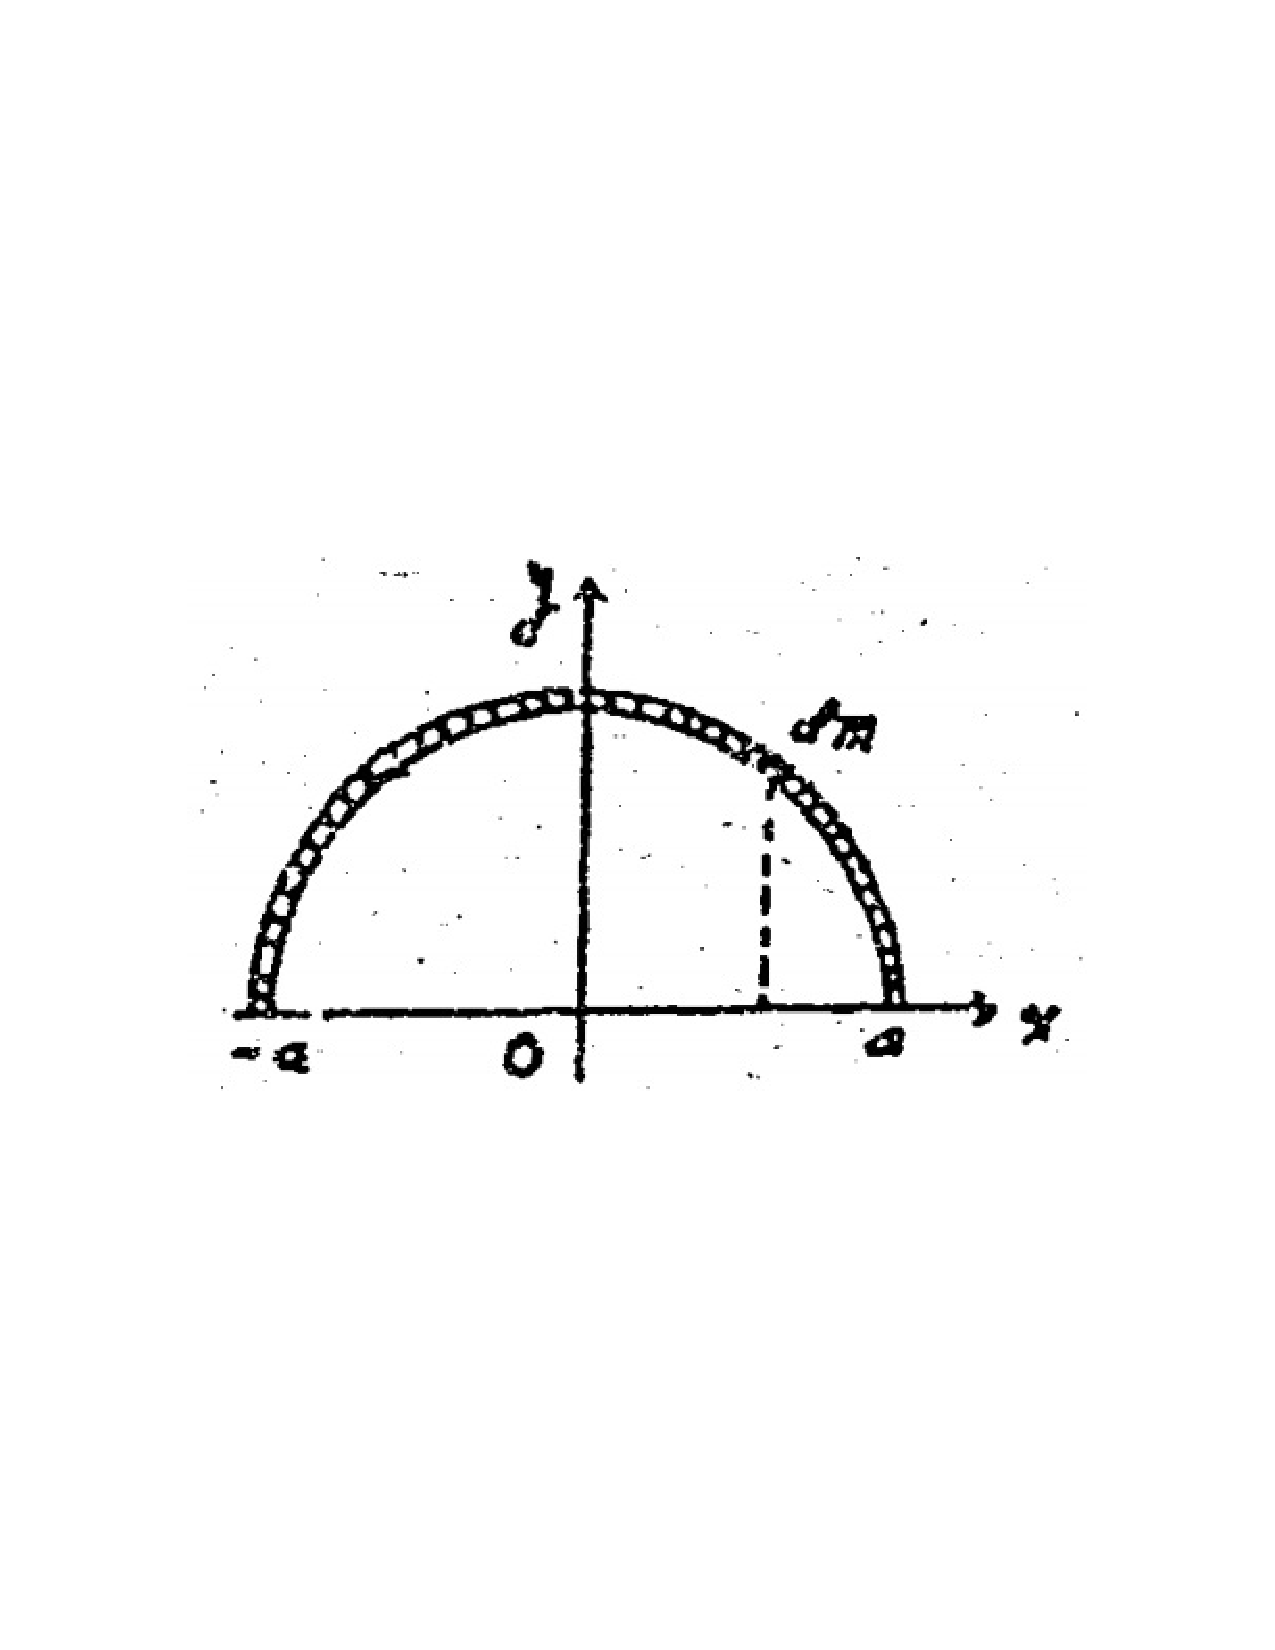
\includegraphics[width=\textwidth]{image}
	\end{minipage}
	
	    
	
	
\end{document}